\documentclass[notitlepage,a4paper,10pt]{article}

% \usepackage{mathpazo} 
\usepackage{mathpazo} 
\usepackage{ngerman} 
\usepackage[latin1]{inputenc} 
\usepackage[T1]{fontenc} 
\usepackage[pdftex]{graphicx} 
\usepackage[pdftex,bookmarks=true,colorlinks,linkcolor=blue,urlcolor=blue,citecolor=blue]{hyperref} 

\sloppy

%opening
\title{Bezahlen im Netz}
\author{https://www.awxcnx.de}
\date{\today}

\hypersetup {
    pdftitle= { Bezahlen im Netz }
    pdfkeywords= {Paysafecard Bitcoin Cashu}
}


\begin{document}
\maketitle


\section{Paypal.com}

Der bekannteste Bezahldienstleister im Internet ist zweifellos \textbf{PayPal.com}. Die Firma wurde von Peter Thiel gegr�ndet, der u.a. den Datensammler Rapleaf.com aufgebaut hat, als einer der Hauptinvestoren die Entwicklung von Facebook ma�geblich mitbestimmt hat und zum Steering Committee der Bilderberg Konferenzen geh�rt. Das Credo von P. Thiel ist eine totale Personalisierung des Internet.\\

Die Nutzung von PayPal.com ist das Gegenteil von anonym. Bei jedem Zahlungsvorgang wird eine Verkn�pfung von pers�nlichen Daten (E-Mail Adresse, Kontoverbindung) und gekauften Waren hergestellt. Die Daten werden an mehr als 100 Firmen �bertragen zum Monitoring der �berweisung.\\

PayPal.com nutzt seine Marktposition f�r die Durchsetzung politischer Interessen der USA. Gem�� der Embargo-Politik der USA werden Internetnutzer in �ber 60 L�ndern ausgesperrt. Internationales Aufsehen erregte die Sperrung der Konten von Wikileaks. Daneben gibt es viele weitere F�lle. Mehr als 30 deutschen Online-H�ndlern wurden die Konten gesperrt \footnote{ \href{http://heise.de/-1320630}{http://heise.de/-1320630}}, weil sie kubanische Produkte (Zigarren, Rum, Aschenbecher) in Deutschland anboten. Die Sperre wurde mit einem amerikanischen Handelsembargo gegen Kuba begr�ndet, das f�r Europ�er belanglos ist.\\

Aufgrund dieser politischen Instrumentalisierung hat \textit{Anonymous} zum Boykott von PayPal.com aufgerufen und an Nutzer appelliert, ihre Accounts bei diesem Bezahldienst zu k�ndigen. 35.000 PayPal-Nutzer sollen dem Aufruf umgehend gefolgt sein.\\

Zuk�nftig m�chte PayPal.com auch in der realen Welt pr�sent sein. Das Bezahlsystem soll die Geldb�rse in zwei Jahren ersetzen, wie Ebay-Chef John Donahoe sagte, nat�rlich mit den �blichen Schn�ffeleien: 
\begin{quote}
\textit{Beim Einsatz von PayPal in den Gesch�ften k�nnten die Einzelh�ndler mehr �ber Vorlieben ihrer Kunden erfahren und sie entsprechend besser bedienen.}
\end{quote} 

\section{Kreditkarten}
Die Kreditkarte ist ein ungeeignetes Zahlungsmittel im Internet. Es erm�glicht das Tracking aller Eink�ufe im Web. Au�erdem kann die Kreditkarte durch Datenverluste beim Online-H�ndler kompromittiert werden. Das passiert �fters:
\begin{itemize}
 \item 400.000 Kunden beim Internetkonzern Unister betroffen (Dez. 2012).\footnote{ \href{http://www.mdr.de/nachrichten/unister130.html}{http://www.mdr.de/nachrichten/unister130.html}} 
 \item 1,5 Millionen Kunden bei Global Payments betroffen (Juni 2012).\footnote{ \href{http://heise.de/-1617091}{http://heise.de/-1617091}} 
 \item Tausenden Nutzer der israelischen Sport-Webseite One.co.il betroffen (Jan. 2012).\footnote{ \href{http://heise.de/-1403584}{http://heise.de/-1403584}}
 \item 24 Millionen Kunden der Amazon-Tochter Zappos betroffen (Jan. 2012).\footnote{ \href{http://www.golem.de/1201/89081.html}{http://www.golem.de/1201/89081.html}}
\end{itemize}
In Carder-Foren kann man diese Kreditkarten f�r 3-10 Euro kaufen.
\subsubsection*{Prepaid-Kreditkarten}
Eine Alternative sind Prepaid-Kreditkarten. An Tankstellen usw. kann man Prepaid-Karten von \textit{mywirecard.com} kaufen. Die Karte kostet ca. 10 Euro und kann bis zu 100,- Euro mit Bargeld beim Kauf aufgeladen werden. Man zahlt also 10\% Security-Bonus.\\

Die Prepaid-Karte muss anschlie�end im Internet aktiviert werden. Dabei wird ein Code per SMS an eine Handynummer gesendet, der auf der Internetseite einzugeben ist. Die Anonymit�t h�ngt also davon ab, ob man ein anonymes Prepaid-Handy nutzt. Man braucht nicht immer die gro�e, richtige Anonymit�t. Wenn ich ein SSL-Zertifikat f�r den Webserver awxcnx.de kaufe, dann ist mehr oder weniger eindeutig klar, wer dahinter steckt. Vergleichbare Anwendungsbeispiele lassen sich f�r den Leser sicher leicht finden.\\

Mit einer Prepaid-Karte kann man einen anonymen PayPal-Account mit fiktiven Daten anlegen. Das er�ffnet M�glichkeiten zur anonymen Nutzung von kommerziellen Angeboten im Internet wie Wuala oder Cilent Circle, die nur Bezahlung via PayPal.com oder Kreditkarte anbieten.\\

Hinweis: Tor Onion Router kann nicht als Anonymisierungsdienst f�r PayPal.com genutzt werden. Paypal.com pr�ft anhand der IP-Adresse den Standort des Nutzers und sperrt den Account, wenn etwas seltsames passiert. Wenn man sich bspw. mit einer deutschen IP-Adresse einloggt und 10min sp�ter mit einer amrikanischen IP-Adresse auf den Account zugreifen m�chte, dann geht PayPal.com von einem Hacker-Angriff aus und sperrt den Account. Mit JonDonym gibt es keine Probleme, wenn man immer die gleiche Mix-Kasakde nutzt.

\section{Bezahlsysteme der Deutschen Bahn}
Am 28. September 2011 ver�ffentlichte die Leaking Plattform Cryptom.org in der Liste der \textit{Online Spying Guides} einen \textit{Leitfaden zum Datenzugriff} der Generalstaatsanwaltschaft M�nchen.\\

Das Dokument zeigt auch, wie das Bezahlsystem der Deutschen Bahn in die �berwachung eingebunden wird. F�r das e-Ticketing der Deutschen Bahn gibt es ein konkretes �berwachungszenario. Durch die Abrechnung �bers Mobiltelefon verf�ge die Deutsche Bahn �ber die Daten s�mtlicher Funkzellen, die der Nutzer durchfahren hat. Diese Daten werden langfristig gespeichert und k�nnen von den Beh�rden auf Gundlage von �100g StPO abgerufen werden. Der Zugriff auf die Reiseprofile ist damit nicht nur bei schweren Straftaten m�glich, sondern auch bei allen Straftaten, die mittels Telekommunikationstechnik begangen wurden.\\

Das Beispiel zeigt, wie bei Nutzung Handy-basierter Bezahlmethoden neue Datenbest�nde anh�ufen. Teilweise k�nnen diese Daten auch als Rechnungsdaten abgerufen werden ohne die juristischen H�rden des Zugriffs auf Kommunikationsdaten.\\

Als Konsequenz kann man Reisenden mit der Deutschen Bahn nur zu anonymen Bargeldzahlungen raten. Wie schnell man pl�tzlich ein \textit{Terrorist} wird, zeigte das Beispiel \textit{Andrej Holm}.

\section{Paysafecard, UKash, Liberty Reserve, Pecunix}
Bei der Nutzung von Alternativen ist man abh�ngig von den Angeboten der Online-H�ndler. Man kann nicht bei allen H�ndlern mit allen Varianten bezahlen und muss als Kunde etwas flexibel sein. 
\begin{itemize}
 \item \textbf{Paysafecard:} entstand aus einem Forschungsprojekt der EU. In vielen Gesch�ften oder Tankstellen kann man Gutscheincodes kaufen. Die Webseite von Paysafecard bietet eine Umkreis-Suche nach Verkaufstellen. Diese Codes kann man �hnlich anonym wie Bargeld im Web zur Bezahlung verwenden (wenn der H�ndler PSC aktzepiert).\\

 Bei der Bezahlung wird man von der Webseite des H�ndlers zur Webseite von Paysafecard weiter geleitet. Dort gibt man den gekauften Code ein und der H�ndler erh�lt die Information, dass die Bezahlung erfolgt ist. Es ist nicht notwendig, dass man einen Gutscheincode genau mit dem geforderten Betrag vorweisen kann. Man kann mehrere Gutscheine f�r eine Bezahlung verwenden oder nur einen Teilbetrag von Gutschein einl�sen. Der Restbetrag bleibt erhalten und kann sp�ter verwendet werden.\\

 Eine Paysafecard ist 12 Monate uneingeschr�nkt g�ltig. Danach werden f�r jeden weiteren Monat 2 Euro vom Guthaben abgezogen. Es ist also sinnvoll, kleinere Guthaben bei Bedarf zu kaufen. Das verhindert auch eine technisch m�gliche Verkettung mehrerer Eink�ufe �ber den gleichen Gutscheincode.\\

 Nach praktischen Erfahrungen von sind die Verk�ufer im Supermarkt, Tankstellen u.�. nicht immer �ber die angebotene M�glichkeit des Verkaufes von Paysafecard Gutscheinen informiert. Hartn�ckig bleiben und die Verk�uferin auf das Paysafecard Symbol im GUI der Kasse hinweisen hilft.\\

Durch Versch�rfung der Sicherheitsvorkehrungen im April 2012 kommt es h�ufig zu gesperrten Gutscheinen, wenn die Gutscheine von verschiedenen IP-Adressen genutzt oder abgefragt werden. Nachfragen beim Support von Paysafecard, wie man die Sperrung der Gutscheincodes vermeiden kann, wurden bisher nicht beantwortet. Wenn ein Gutschein gesperrt wurde, muss man sich an den Support von Paysafecard wenden. Restbetr�ge kann man sich unter Angabe der eigenen Kontonummer erstatten lassen.\\

Aufgrund des Gesetzes gegen Geldw�sche ist Paysafecard gezwungen, die Anonymit�t des Zahlungsmittels einzuschr�nken. Deutsche Nutzer sollen (aber m�ssen nicht) auf der Website unter \textit{``My PaySafaCard``} einen Account erstellen und k�nnen diesen Account mit Gutscheincodes aufladen. Wer mehr als 100,- Euro pro Monat nutzen m�chte, muss sich mit Ausweisdokumenten identifizieren. Probleme mit gesperrten Gutscheinen soll es dann nicht geben.\\

Eine Nutzung von mehreren Gutscheinen mit Restbetr�gen f�r einen Bezahl�vorgang ist seit Sept. 2012 NICHT mehr m�glich! Restbetr�ge kann man sich unter Angabe der Kontonummer erstatten lassen. Damit wird die Anonymit�t des Zahungsmittels leider etwas ausgehebelt. Passende Paysafecards gibt es nicht immer, es gibt nur Gutscheine f�r 10, 15, 20, 25, 30, 50 oder 100 Euro.

\item \textbf{UKash:} funktioniert �hnlich wie Paysafecard, bietet aber nicht ganz so viele Verkaufsstellen in Deutschland. Im Gegensatz zu Paysafecard sind keine Probleme mit gesperrten Gutschein�codes bekannt. Au�erdem wird man bei UKash nicht zur Einrichtung eines Accounts gedr�ngt. Die Nutzung ist damit anonymer, als mit Paysafecard.\\

Mit UKash Codes kann man Konten bei Liberty Reserve (via eCardOne) oder cashU aufladen. Dabei muss man such jedoch mit einer Kopie des Ausweises oder Pass authentifizieren.

\item \textbf{Liberty Reserve:} ist ein weiterer vertrauensw�rdiger Bezahldienstleister im Web. Man muss einen Account erstellen, die Angaben werden aber nicht �berpr�ft. Lediglich die E-Mail Adresse muss g�ltig sein. Bei Liberty Reserve werden getrennte Konten f�r Dollar und Euro gef�hrt. Man muss darauf achten, welche W�hrung der Webshop akzeptiert.\\

Aufladen des Accounts mit Guthaben ist �ber verschiedene Exchanger m�glich. Bei eCardOne kann man den Liberty Reserve Account mit UKash Codes aufladen, muss sich daf�r aber neuerdings mit einer Ausweiskopie identifizieren. Da Liberty Reserve ein sehr gro�er Bezahldienstleister ist, gibt es viele unseri�se Anbieter, die ein Aufladen des Account versprechen aber nur die Zahlung einsacken und nichts dem Liberty Reserve Accout gutschreiben (z.B. UCash Exchanger) oder Geb�hren von mehr als 50\% der Zahlung nehmen (z.B. cashvoucers). 

Nutzen Sie nur die auf der Website von Liberty Reserve gelisteten und verifizierten Exchanger!

\item \textbf{Pecunix:} wickelt Bezahlungen in Gold ab. Die Geldbetr�ge werden bei Bezahlung automatisch in Gold umgerechnt. Um mit Pecunix zu bezahlen, ist ein Account zu erstellen, bei dem ebenfalls lediglich die E-Mail Adresse g�ltig sein muss. Als einziger Bezahldienstleister kann Pecunix den gesamten E-Mail Verkehr zu den Nutzern mit OpenPGP verschl�sseln. Man kann seinen eigenen OpenPGP-Schl�ssel im Account hochladen und die Option zur Verschl�sselung aktivieren.\\

Um mit Pecunix bezahlen zu k�nnen, muss man eGold kaufen. Auf der Webseite von Pecunix findet man einen Liste von Exchangern.

\item \textbf{cashU:} ist ein Bezahlservice, der haupts�chlich in der arabischen Welt verwendet wird. Registrieren kann man sich \textit{wie man will} und die Konten bleiben un�berpr�ft bestehen. Die cashU W�hrung l�sst sich auf der Webseite durch UKash Codes aufladen, wenn man sich mit einer Kopie des Ausweises identifiziert. Einen anderen Weg habe ich von Deutschland aus noch nicht gefunden.
\end{itemize}

\subsection{Anonyme Online-Zahlungen vor dem Aus?}
Die Bundesregierung bereitete unter dem Deckmantel des Kampfes gegen Geldw�sche ein Gesetz vor, das f�r anonyme Bezahlungen im Internet das Aus bedeutet h�tte. K�nftig sollen Verkaufsstellen von Paysafecards und UKash Vouchers die K�ufer identifizieren und die Daten f�r eine m�gliche Pr�fung 5 Jahre bereithalten. Im Gegensatz zu Bareinzahlungen, die statt bisher ab 15.000 Euro zuk�nftig ab 1.000 Euro berichtspflichtig werden, sollten f�r E-Geld keine Mindestgrenzen gelten.\footnote{ \href{http://heise.de/-1269409}{http://heise.de/-1269409}}\\

Nach Ansicht von Udo M�ller (Paysafecard-Gesch�ftsf�hrer) w�ren diese Anforderungen auch f�r die Vertriebsstruktur das AUS. 95\% der Partner wie Tankstellen, Gesch�fte usw. w�rden unter diesen Bedingungen den Verkauf von Paysafecard Gutscheinen und UKash Vouches einstellen.\\

Unklar ist, wie die bei E-Geld �blichen Kleinbetr�ge in nennenswertem Umfang f�r Geldw�sche genutzt werden k�nnen. Die Regierung hat daf�r keine sinnvolle Erkl�rung geliefert. Nach den vom BKA vorgelegten Zahlen zum Missbrauch von Prepaidkarten zur Geldw�sche ist der Missbrauch sehr gering. Nur in 94 von 14.000 Verdachtsf�llen, die gemeldet wurden, spielten Prepaidkarten eine Rolle. Das sind 0,7\% aller Verdachtsf�lle. Der Bundesdatenschutzbeauftragte Schaar hat sich gegen den Entwurf ausgesprochen:
\begin{quote}
\textit{Ich appelliere an den Gesetzgeber, den �berzogenen Ansatz der neuen Vorschl�ge entsprechend zu korrigieren.}
\end{quote} 

Die 82. Konferenz der Datenschutzbeauftragten Ende September 2011 verfasste zu diesem Gesetzentwurf eine Stellungnahme:
\begin{quote}
\textit{Nach den vorgesehenen Regelungen w�rden noch mehr personenbezogene Daten unbescholtener B�rgerinnen und B�rger erfasst und ganz �berwiegend anlasslos gespeichert. Dies steht in Widerspruch zur Rechtsprechung des Bundesverfassungsgerichts.}
\end{quote}

Am 01. Dez. 2011 hat der Deutsche Bundestag das Gesetz in einer etwas entsch�rften Version beschlossen. F�r den Kauf von Prepaidkarten bis 100 Euro ist keine Identifizierung der K�ufer n�tig. F�r Prepaidguthaben von mehr als 100 Euro sind die K�ufer zu identifizieren. Die Daten sind 5 Jahre lang zu speichern. Der Bundesdatenschutzbeauftragte kommentierte die Verabschiedung des Gesetzes u.a. mit folgenden Worten:
\begin{quote}
\textit{So begr��enswert es ist, dass der anonyme Erwerb von E-Geld damit nicht generell abgeschafft wird, so kritisch sehe ich die nach wie vor bestehende Tendenz, individuelles Handeln in immer st�rkerem Ma�e zu registrieren\dots} \\
 
\textit{Die Diskussion �ber Identifikationspflichten - vor allem bei der Inanspruchnahme des Internets - ist damit aber sicherlich noch nicht beendet.}
\end{quote}


\section{Bitcoin}
Bitcoin ist eine digitale Peer-2-Peer W�hrung ohne zentrale Verwaltung. Sie ist unabh�ngig von der Geldpolitik einer Zentralbank und entwickelt sich marktgetrieben durch die Aktivit�ten der Teilnehmer, die Bitcoin als Zahlungsmittel akzeptieren oder verwenden.\\

Die Wurzeln der �konomischen Theorie dieser virtuellen W�hrung liegen in der \textit{Austrian school of economics}, die von den �konomen Eugen v. B�hm-Bawerk, Ludwig Mises und Friedrich A. Hayek entwickelt wurde. Die �konomen kritisieren das gegenw�rtige System des Fiatgeldes der Zentralbanken. Sie sehen in den massiven, politisch motivierten Interventionen der Zentralbanken in den Geldumlauf eine wesentliche Ursache f�r den Krisenzyklus. Als Ausweg empfehlen sie eine Internationalisierung der W�hrungen und die R�ckkehr zum Goldstandard.\\

Gegenw�rtig ist Bitcoin die popul�rste Umsetzung einer W�hrung in Anlehnung an die Konzepte der \textit{Austrian school of economics}. Die Software l�st mit kryptografischen Methoden vor allem zwei Probleme:

\begin{enumerate}
 \item Das Kopieren und mehrfache Verwendung der Bits und Bytes, die ein Coin repr�sentieren, ist nicht m�glich.
 \item Die Gesamtmenge der verf�gbaren Coins ist limitiert.
\end{enumerate}

Darauf aufbauend kann Bitcoin als Bezahlmethode verwendet werden. 
\begin{itemize}
 \item Bitcoins lassen sich in reale W�hrungen hin- und zur�cktauschen. Der Kurswert der Bitcoins beim Tausch gegen reale W�hrungen (z.B. Euro) ergibt sich dabei ausschlie�lich aus dem Markt.
 \item Die Bezahlungen k�nnen relativ schnell am PC abgewickelt werden. Es dauert in der Regel nur 1-2h, bis das Bitcoin Netzwerk eine Transaktion hinreichend best�tigt hat.
 \item Au�erdem hat Bitcoin einen Inflationsschutz. Neue Bitcoins werden nach einem festen Schema generiert und die Gesamtzahl ist limitiert.
\end{itemize}

Viele Dienste im Netz akzeptieren Bitcoins als Bezahlung. Eine �bersicht findet man im Bitcoin Wiki \footnote{ \href{https://en.bitcoin.it/wiki/Trade}{https://en.bitcoin.it/wiki/Trade}}. Man kann Musik, E-Books, Web- und Mailhosting oder Anonymisierungsdienste / VPN-Anbieter mit Bitcoins bezahlen. Der Kurs wird dabei von jedem Anbieter selbst festgelegt. Dabei kann es vorkommen, dass Anbieter vom mittleren Tauschkurs abweichen.\\

Um mit Bitcoins zu bezahlen, braucht man selbst ein paar Bitcoins. Diese kann man auf verschiedenen Markpl�tzen gegen reale W�hrung kaufen oder man bietet selbst Dienst�leistungen gegen Bitcoins als Bezahlung an. Die Markpl�tze dienen dabei nur zur Anbahnung der Transaktionen \textit{Geld gegen Bitcoin}. Der Austausch des reales Geldes erfolgt in der Regel auf direktem Weg zwischen den Beteiligten.\\

In der Regel k�nnen die Markpl�tze/Exchanger die gekauften Bitcoins f�r die Nutzer auch verwalten. Das vereinfacht die Nutzung von Bitcoin als Zahlungsmittel, da eine Installation von Software nicht zwingend n�tig ist. Die erworbenen Bitcoins k�nnen aber auch auf den eigenen PC transferiert und lokal verwaltet werden. Hierf�r muss ein Bitcoin Client installiert werden.\\

\subsection{Exchanger / Marktpl�tze}
Man kann Bitcoin komplett ohne Installation einer Software nutzen. Es gibt Webdienste (die sogenannten Exchanger oder Markpl�tze), die den Handel mit Bitcoins zwischen den Personen einleiten und eine Bitcoin Brieftasche (eWallet) f�r Nutzer bereitstellen. Die Exchanger verifizieren die Identit�t der Nutzer. Eine anonyme Nutzung ist nicht m�glich. Hinweise zum anonymen Kauf von Bitcoins findet man weiter unten im Abschnitt \textit{Anonymit�t von Bitcoin}.\\

Eine �bersicht zu den Marktpl�tzen findet man auch im Bitcoin Wiki \footnote{ \href{https://en.bitcoin.it/wiki/Buying\_bitcoins}{https://en.bitcoin.it/wiki/Buying\_bitcoins}}. F�r den Einstieg gef�llt mir \textbf{\href{https://www.bitcoin.de}{www.bitcoin.de}} sehr gut. Die Webseite wird professionell betreut, bietet in einer �ber�sichtlichen Struktur alle n�tigen Informationen f�r Kaufen, Verkaufen und die Verwaltung der eigene Bitcoins und ist f�r die ersten Schritte gut geeignet. Allerdings ist der Dienst nicht ganz kostenfrei. Es wird eine Geb�hr von 1\% f�r den Handel mit Bitcoins erhoben.\\

Die Anmeldung bei Bitcoin.de erfordert die Angabe einer E-Mail Adresse und einer Bank�verbindung. Die Bankverbindung wird durch eine einmalige �berweisung von 1 Cent verifiziert. Tempor�re E-Mail Adressen sollten nicht genutzt werden, da bei jeder Transaktion Informationen per Mail gesendet werden. Man kann zus�tzliche Zahlungsm�glichkeiten wie Liberty Reserve oder Money Bookers nutzen.\\ 

\textbf{Bitcoins kaufen:} Im Markbereich stehen in einer Liste mehrer Verkaufsangebote. Durch Klick auf den Link \textit{Kaufen} kann man ein Kaufangebot annehmen. Sie erhalten ein E-Mail mit den Daten f�r die Bezahlung. �berweisen Sie dem Verk�ufer das Geld und best�tigen Sie die �berweisung auf der Webseite innerhalb von 12h. Wenn der Verk�ufer den Zahlungseingang best�tigt, erhalten Sie die Bitcoins. Wenn kein passendes Angebot zu finden ist, k�nnen Sie ein Kaufangebot einstellen und auf Angebote warten.\\

Wichtig: Sie senden dem Verk�ufer den Kaufpreis abz�glich 0.5\% und erhalten daf�r Bitcoins abz�glich 1\% des Kaufangebotes. Somit teilen sich K�ufer und Verk�ufer die Marktgeb�hr von 1\% jeweils zur H�lfte. Ein Rechenbespiel: 
\begin{itemize}
 \item Das Angebot lautet: 1 BTC f�r 40,00 Euro.
 \item Der K�ufer �berweist 39,80 Euro an den Verk�ufer.
 \item Er erh�lt daf�r 0,99 BTC auf seinem Konto.
\end{itemize}

Die f�r ihre Transaktion g�ltigen Zahlen werden jeweils bei Annahme des Kaufangebotes und in der E-Mail angezeigt. Die Kontodaten des Verk�ufers erhalten Sie ebenfalls per E-Mail.\\

\subsection{Bitcoin Software}
Wenn man einem externen Webserver nicht vertraut, kann man seine Bitcoins lokal auf dem eigenen Rechner oder Smartphone verwalten. Daf�r braucht man einen Bitcoin Client

\subsubsection*{Bitcoin-Qt}
Botcoin-Qt\footnote{ \href{http://bitcoin.org/en/download}{http://bitcoin.org/en/download}} ist der Standard Client des Bitcoin Projektes. Er ist einfach bedienbar, bietet eine �bersicht �ber alle Transaktionen und kann beliebig viele Adressen verwalten.\\

Ein Nachteil f�r Gelegenheitsnutzer ist der st�ndige Download der gesamten Blockchain (des \textit{ewigen Logfiles}). Die Down�load�seite weist darauf hin, dass die erste Initialisierung bis zu einem Tag dauern kann. Wenn man nach 3-4 Wochen Pause wieder einmal mit Bitcoins bezahlen m�chte, dann ben�tigt Bitcoin-Qt ein bis zwei Stunden, um arbeitsbereit zu sein.

\subsubsection*{Electrum}
Der leichtgewichtige Bitcoin Client Electrum\footnote{ \href{http://electrum.org/}{http://electrum.org/}} ist eine Alternative f�r Gelegenheitsnutzer. Er �berl�sst die Hauptarbeit speziellen Servern im im Netz und ben�tigt die Blockchain nicht. Trotzdem ist sichergestellt, dass die privaten Schl�ssel ausschlie�lich in der Verf�gung des Anwenders liegen. Die Installation f�r unterschiedliche Betriebssysteme ist auf der Down�load�seite\footnote{ \href{http://electrum.org/download.html}{http://electrum.org/download.html}} beschrieben.\\

\begin{figure}[tb]
\begin{center}
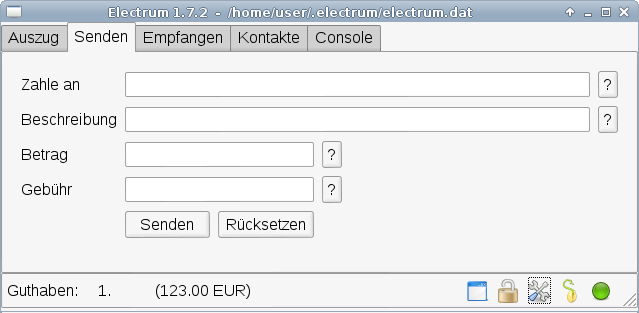
\includegraphics[scale=0.55]{../screenshots/electrum2.png}
\caption{Hauptfenster von Electrum}
\label{abb:electrummain}
\end{center}
\end{figure}

Die Oberfl�che ist einfach gehalten. F�r die �bersicht der Transaktionen, zum Senden und Empfangen sowie eine einfache Adressliste gibt es Reiter im Hauptfenster (Bild \ref{abb:electrummain}).\\

Alle Transaktionen werden in der Blockchain gespeichert. Sie k�nnen mit dem \textit{Seed} aus dem \textit{ewigen Logfile} rekonstruiert werden. Ein vollst�ndiges Backup der Konfiguration ist nicht n�tig. Man ben�tigt nur den Seed, der wie eine lange Passphrase aus zw�lf Worten besteht. F�r ein Backup des Seed klickt man auf zweite Symbol von rechts in der Statusleiste und speichert die Passphrase (z.B. in einer verschl�sselten Passwortdatenbank wie KeepassX). Mit dem QR-Code kann man den Seed schnell auf ein Smartphone �bertragen.\\

\begin{figure}[tb]
\begin{center}
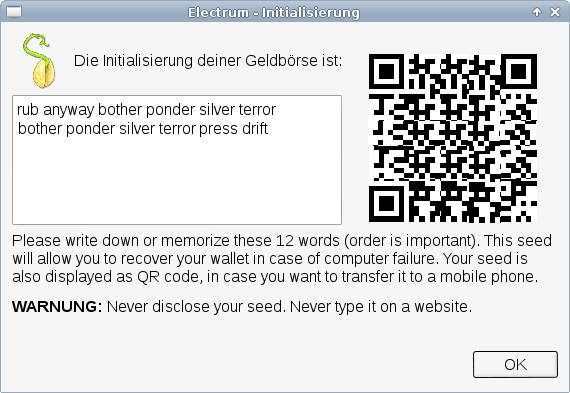
\includegraphics[scale=0.55]{../screenshots/electrum3.png}
\caption{Seed exportieren}
\label{abb:electrumseed}
\end{center}
\end{figure}

Die Netzwerkeinstellungen �ffnet man mit einem Klick auf das rechte Icon in der Statusleiste, dass �blicherweise ein gr�ner Punkt ist. Hier kann man festlegen, welchen Server man f�r die rechenintensiven Aufgaben nutzen m�chte. Der Server kann aus der Liste frei gew�hlt werden. Es werden keine Accountdaten auf dem Server gespeichert.\\

Au�erdem kann man in den Netzwerkeinstellungen den Proxy konfigurieren. Da Electrum nur geringen Datenverkehr verursacht, ist eine sinnvolle Kombination mit den Anonymisierungs�diensten Tor oder JonDonym m�glich. Das verhindert eine zuk�nftige Deanonymiserung des Nutzers durch Analyse des ewigen Logfiles. Die Proxy Einstellungen k�nnen auch beim Start des Programms als Parameter �bergeben werden:
\begin{itemize}
 \item Um den Datenverkehr von Electrum mit den Premiumdiensten von JonDonym zu anonymisieren, startet man das Programm mit folgenden Proxy-Parametern:
 \begin{verbatim}
    electrum --proxy=http:127.0.0.1:4001
 \end{verbatim} 
 \item Wenn man Tor Onion Router nutzen m�chte (TorBrowserBundle), dann nimmt man:
 \begin{verbatim}
    electrum --proxy=socks5:127.0.0.1:9150
 \end{verbatim}
\end{itemize}

Die Server f�r den rechenintensiven Part werden durch Spenden finanziert. Die Betreiber sind f�r eine kleine Spende in Bitcoins dankbar. Die Spendenadresse f�r den aktuell genutzten Server findet man auf dem Reiter \textit{Console} im Hauptfenster.

\subsection{Anonymit�t von Bitcoin}
�ber die Anonymit�t von Bitcoin gibt es viele Missverst�ndnisse. So wie jeder Geldschein eine eindeutige Nummer hat und verfolgt werden kann, ist es einem potenten Beobachter auch m�glich, Bitcoin Zahlungen zu verfolgen.\\

Alle Bitcoin Transaktionen werden im \textit{ewigen Logfile} protokolliert, das �ffentlich zug�nglich ist. Das ist kein Designfehler sondern notwendig, um double spending zu verhindern. Forscher der TU Darmstadt haben auf dem 28C3 eine Analyse des \textit{ewigen Logfile} von Bitcoin vorgestellt \footnote{ \href{http://events.ccc.de/congress/2011/Fahrplan/events/4746.en.html}{http://events.ccc.de/congress/2011/Fahrplan/events/4746.en.html}}. Eine weitere Analyse wurde von D. Ron und A. Shamir publiziert \footnote{ \href{http://eprint.iacr.org/2012/584}{http://eprint.iacr.org/2012/584}}. Beide Analysen konnten scheinbar unabh�ngige Bitcoin Adressen zusammen f�hren und die IP-Adressen von Nutzern ermitteln. Dazu z�hlen beispielsweise Spender, die an Wikileaks via Bitcoin gespendet haben. Au�erdem wurden Zahlen zur Bitcoin Nutzung von Wikileaks als Beispiel ver�ffentlicht. Bis M�rz 2012 nutzte Wikileaks 83 Bitcoin Adressen und erhielt 2605.25 BTC von Unterst�tzern.\\

Die Forscher kommen zu dem Schluss, dass die Anonymit�t von Bitcoin geringer ist, als eine einfache Bank�berweisung. Informationen zu Bank�berweisungen kann man nicht \textit{einfach so} bekommen. as Bankgeheimnis verwehrt vielfach den Zugriff auf die Konto�informationen. Die Bitcoin Transaktionen kann jeder analysieren, der �ber die n�tige Rechenleistung verf�gt.\\

Die CIA hat nach eigenen Aussagen Bitcoin als Zahlungsmittel \textit{bereits auf dem Radar}. Im Juni 2011 wurde Gavin Andresen (ein f�hrender Bitcoin Entwickler) ins CIA-Haupquartier zu einer Pr�sentation eingeladen. Auch das US-Milit�r sucht(e) bereits einen Anti-Terror Finanzexperten mit Bitcoin Erfahrung. Die Europ�ische Zentralbank (EZB) sieht laut einem Bericht von Okt. 2012 in Bitcoin eine Gefahr, da es au�erhalb der Kontrolle der Zentralbanken l�uft. Die EZB empfiehlt eine intensivere Beobachtung. Es gibt also viele Gr�nde, m�glichst anonym zu bleiben.

\subsubsection*{Bitcoin anonym nutzen}
Da der gesamte System von Bitcoin auf Informationsaustausch im Internet basiert, ist es mit Anonymisierungsdiensten m�glich, Bitcoin auch vollst�ndig anonym zu nutzen. Dabei sind folgende Punkte zu beachten:

\begin{description}
 \item[Bitcoin-Brieftasche anonym verwalten:] 
  Man kann einen Webservice verwenden und mit den Anonymisierungs�diensten \textit{JonDo+JonDoFox} oder dem \textit{TorBrowserBundle} das eWallet anonym auf den Servern verwalten.
 \begin{itemize}
  \item Blockchain.info\footnote{ \href{https://www.blockchain.info/wallet}{https://www.blockchain.info/wallet}} bietet die Verwaltung eines anonymen eWallet auf dem Webserver und erfordert keine pers�nlichen Angaben bei der Registrierung.
  \item StrongCoin.com\footnote{ \href{https://www.strongcoin.com}{https://www.strongcoin.com}} erfordert die Angabe einer E-Mail Adresse bei der Registrierung. Wegwerfadressen werden akzeptiert. Das Webinterface ist f�r Smartphones geeignet.
  \item OnionBC ist ein anonymer eWallet Service, der nur als Tor Hidden Service unter \href{http://6fgd4togcynxyclb.onion/}{6fgd4togcynxyclb.onion} erreichbar ist. (Ich bin immer etwas skeptisch bei Tor Hidden Services. Wenn man nicht weiss, wer den Dienst betreibt, kann es sich oft um Scam handeln. TORwallet hat sich z.B. als Scam herausgestellt.)
 \end{itemize}
 
Wenn man einem Webdienst nicht vertrauen m�chte, kann man den Bitcoin Client \textit{Electrum}\footnote{ \href{http://electrum.org/index.html}{http://electrum.org}} installieren und den Datenverkehr mit Tor oder JonDonym anonymisieren. Electrum �ber�l�sst die Hauptarbeit speziellen Servern und muss deshalb nicht das \textit{ewige Logfile} st�ndig aktualisieren. Das reduziert den Datenverkehr und erm�glicht eine sinnvolle Kombination mit JonDonym oder Tor. Die privaten Schl�ssel bleiben aber immer auf dem eigenen Rechner.\\

Um den Datenverkehr von Electrum mit den Premiumdiensten von JonDonym zu anonymisieren, startet man das Programm mit folgenden Proxy-Parametern:
\begin{verbatim}
    electrum --proxy=http:127.0.0.1:4001
\end{verbatim} 
Wenn man Tor Onion Router nutzen m�chte (TorBrowserBundle), dann startet man das Programm mit folgenden Proxy-Parametern:
\begin{verbatim}
    electrum --proxy=socks5:127.0.0.1:9150
\end{verbatim} 
Die Installation von JonDo oder Tor ist im Kapitel \textit{Anonymisierungsdienste} beschrieben.

\item[Bitcoins anonym kaufen:]
Man kann beim Kauf von Bitcoins die Angabe eines Bankkontos oder anderer identifizierender Informationen vermeiden.
\begin{itemize}
 \item Auf der Webseite LocalBitcoins.com\footnote{ \href{https://localbitcoins.com/}{https://localbitcoins.com/}} findet man weitere Anbieter in der Umgebung, die Bitcoins gegen Cash mit pers�nlicher Geld�bergabe verkaufen.
 \item Im IRC Channel \#bitcoin-otc im Freenode Netz kann man beliebige Formen der Geld�bergabe mit dem Verk�ufer vereinbaren.
 \item In Berlin trifft sich die Bitcoin Community an jedem ersten Donnerstag im Monat im \textit{room 77} (Graefestr. 77, 10967 Berlin-Kreuzberg). Dort findet immer jemanden, der Bitcoins gegen Bargeld verkauft.
 \item Wer den Anonymisierungsdienst JonDonym nutzt, kann im Bitcoin Shop der JonDos GmbH \footnote{ \href{https://shop.anonymous-proxy-servers.net/bin/btc-shop}{https://shop.anonymous-proxy-servers.net/bin/btc-shop}} anonym kaufen und mit Paysafecard bezahlen (wenn Coins im Shop vor�handen sind). Damit kann man auch Restbetr�ge von Paysafecards verwenden.
\end{itemize}

\item[Bitcoins als Zahlungsmittel verwenden:]
 Beim Einkauf virtueller G�ter (z.B. JonDonym Premium Codes oder eBooks, die per E-Mail zugestellt werden) gibt es keine weiteren Probleme. Muss man beim Kauf realer G�ter eine Lieferadresse angeben, dann sollte man ein anderes Bitcoin eWallet verwenden als f�r die anonyme Bezahlung virtueller G�ter. Anderenfalls k�nnten auch  die anonymen Zahlungen deanonymisiert werden.\\

\item[Mixing-Services?] Im Bitcoin-Wiki werden Mixing-Services wie Blockchain Mixing Service\footnote{ \href{https://blockchain.info/wallet/send-anonymously}{https://blockchain.info/wallet/send-anonymously}} oder Cleanbit.org\footnote{ \href{http://www.cleanbit.org/}{http://www.cleanbit.org/}} empfohlen, um die Spuren einer Transaktion zu verwischen. Die Analyse von D. Ron und A. Shamir l�sst vermuten, dass diese Mixing-Services mit entsprechendem Aufwand analysiert werden k�nnten und zuk�nftig einen potenten Angreifer nicht von einer Verfolgung der Transaktionen abhalten k�nnen.

 \end{description}
 

\end{document}